\documentclass[a4paper]{article}
\usepackage{amsfonts}
\usepackage{amsmath}
\usepackage{amssymb}
\usepackage{graphicx}     

\begin{document}
  
\noindent \large Auteur: Raj Shah \\
\noindent \large Studierichting: Informatica\\
\noindent \large Oefeningenreeks 5G nr. 5.3 \\

\medskip

\normalsize

$f(x) = \cos x + \sin x$ en $g(x) = \cos x - \sin x$ op interval $\left[0, \dfrac{\pi}{4}\right]$\\

$ V = \pi \displaystyle\int_{0}^{\tfrac{\pi}{4}}\left((\cos x + \sin x)^2 - (\cos x - \sin x)^2\right)dx$\\

$ = \pi \displaystyle\int_{0}^{\tfrac{\pi}{4}} \left((\cos^2 x + 2\sin x\cos x + \sin^2 x) - (\cos^2 x - 2\sin x\cos x + \sin^2 x)\right)dx$\\

$ = \pi \displaystyle\int_{0}^{\tfrac{\pi}{4}} 4\sin x\cos x dx = 2\pi \displaystyle\int_{0}^{\tfrac{\pi}{4}} 2\sin x\cos x dx$ \\

$ = 2\pi \displaystyle\int_{0}^{\tfrac{\pi}{4}} \sin 2x dx$ \\

$ = 2\pi \left[\dfrac{-\cos 2x}{2}\right]_{0}^{\tfrac{\pi}{4}} = \dfrac{2\pi}{2} \cdot \left(-\left(\cos \dfrac{\pi}{2} - \cos 0\right)\right)$ \\

$ = \pi \cdot (0 + 1) = \pi $\\


\begin{figure}[h]
\centering
    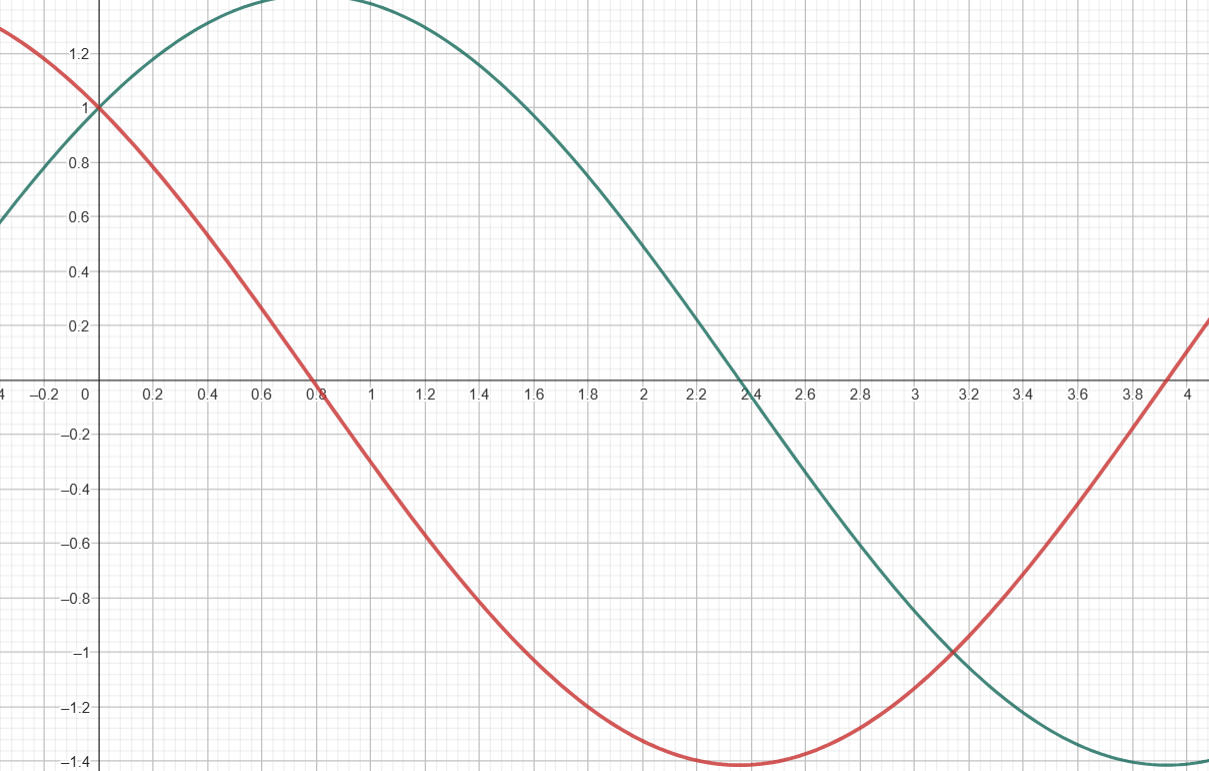
\includegraphics[width=\linewidth]{5G-5.3-raj.shah.INF.png}\\
\end{figure}

\begin{thebibliography}{999}
%\bibitem{a} Referentie
\end{thebibliography}
\end{document} 
